%% Flight Delay Prediction --- Advanced Machine Learning Phase (Project 21, Team T022)
%% IEEE conference-style report. Compiles with pdflatex (IEEEtran class).
%% Build:  pdflatex main  ->  pdflatex main   (run twice for references/labels)
%% Or upload this folder to Overleaf and select pdfLaTeX.

\documentclass[conference]{IEEEtran}
\IEEEoverridecommandlockouts

\usepackage{graphicx}
\usepackage{amsmath}
\usepackage{amssymb}
\usepackage{booktabs}
\usepackage{array}
\usepackage{url}
\usepackage[hidelinks]{hyperref}
\usepackage{xcolor}

\graphicspath{{figures/}}

% Convenience macros for feature names with underscores.
\newcommand{\code}[1]{\texttt{#1}}

\begin{document}

\title{Flight Delay Prediction via Gradient Boosting and\\ Calibrated Classical Learning: A Leakage-Safe Pipeline\\ with an Offline Rescheduling What-If Analysis}

\author{
\IEEEauthorblockN{Samiksha Jangid}
\IEEEauthorblockA{Data Pipeline \&\\ Leakage Prevention\\ Team T022, Section C}
\and
\IEEEauthorblockN{Rashmi Anand}
\IEEEauthorblockA{Exploratory Analysis \&\\ Feature Engineering\\ Team T022, Section C}
\and
\IEEEauthorblockN{Ankit Raj Singh}
\IEEEauthorblockA{Logistic Regression\\ Baseline\\ Team T022, Section C}
\and
\IEEEauthorblockN{Shubhaang Kataruka}
\IEEEauthorblockA{XGBoost \&\\ Hyperparameter Tuning\\ Team T022, Section C}
\and
\IEEEauthorblockN{Lakshya}
\IEEEauthorblockA{Evaluation \&\\ Calibration\\ Team T022, Section C}
}

\maketitle

\begin{abstract}
We predict whether a scheduled flight will arrive at least fifteen minutes late,
using only information available before departure, and study whether the
resulting probabilities can support proactive rescheduling. Using one year of
2013 US flights originating from the three major New York airports, we build a
leakage-safe pipeline whose defences operate at three levels: a pre-departure
feature allowlist, historical delay statistics aggregated from prior calendar
dates only, and a strictly chronological train/validation/test split. We
engineer temporal (cyclic), route, prior-date historical and schedule-based
airport-congestion features, and train
a class-balanced Logistic Regression and a tuned XGBoost classifier. Probabilities
are calibrated on a held-out late-training window (isotonic regression, selected
by validation Brier score), and a single operating threshold per model is frozen
on validation before one-time evaluation on the held-out test set. XGBoost is the
stronger held-out candidate (test PR-AUC $0.338$, ROC-AUC $0.599$) but absolute
discrimination is modest, and a proper-score audit shows the calibrated
probabilities are not convincingly better than a prevalence baseline. We then
derive an offline cost-sensitive rescheduling rule with a closed-form net-benefit
and a cost-optimal action threshold $\tau^\star = C_a/(r\,C_d)$, and report a
sensitivity analysis: a model-guided rule beats inaction only when interventions
are cheap relative to a delay, and XGBoost has the more favourable cost-sensitivity
profile over the meaningful cost range. We emphasise honest reporting of limitations and treat
this phase as the calibrated baseline for a subsequent deep-learning extension.
\end{abstract}

\begin{IEEEkeywords}
flight delay prediction, data leakage, probability calibration, gradient
boosting, class imbalance, cost-sensitive decision analysis, decision curve
analysis.
\end{IEEEkeywords}

\section{Introduction}
Flight delays impose large and cascading costs on passengers, carriers and the
air-traffic system. Most of the operational value of a delay prediction is
realised \emph{before} the aircraft leaves the gate, when swaps, buffers and
re-bookings are still possible. This motivates a strict problem definition: a
prediction made at the scheduled-departure decision point may use only
information that is genuinely available at that moment.

The central methodological risk in such a task is \emph{data leakage}---allowing
information unavailable at prediction time to influence training or evaluation,
which inflates apparent accuracy and produces a model that fails in deployment.
A second risk is \emph{miscalibration}: a classifier may rank flights well yet
emit probabilities that do not correspond to real-world frequencies, which is
fatal for any downstream decision rule that thresholds a probability.

This report, covering the Advanced Machine Learning phase of the project, makes
four contributions. First, a leakage-safe data pipeline with three independent
defences (Section~\ref{sec:method}). Second, documented and unit-tested feature
engineering, including a cyclic time encoding and prior-date historical
aggregates (Section~\ref{sec:features}). Third, a calibrated, chronologically
fair evaluation of a Logistic Regression baseline against a tuned XGBoost model,
with a frozen one-time test (Section~\ref{sec:results}). Fourth, an offline
rescheduling what-if analysis built on explicit cost assumptions, including the
cost-optimal operating threshold and a sensitivity study
(Section~\ref{sec:resched}). Throughout, we favour transparent reporting of
weaknesses over optimistic claims.

\section{Related Work}
\label{sec:related}
\textbf{Flight delay prediction.} Delay modelling spans queuing and network
propagation models~\cite{rebollo} through to data-driven machine learning on
large operational records~\cite{gui}. The US Bureau of Transportation Statistics
(BTS) defines the fifteen-minute threshold for a ``delayed'' flight and publishes
the on-time performance data that underpins much of this
literature~\cite{bts}. Our work adopts the BTS threshold and the pre-departure
constraint but deliberately restricts itself to a compact, reproducible
single-year dataset for the baseline phase.

\textbf{Gradient boosting.} Gradient-boosted decision trees, and XGBoost in
particular~\cite{xgboost}, are strong tabular learners that capture non-linear
feature interactions with modest tuning, making them a natural comparator to a
linear baseline.

\textbf{Probability calibration.} Guo \emph{et al.}~\cite{guo} show that modern
classifiers are frequently miscalibrated and that post-hoc recalibration is
often necessary. Classic post-hoc methods include Platt scaling (a sigmoid
fit)~\cite{platt} and isotonic regression (a non-parametric monotone
map)~\cite{zadrozny}; Niculescu-Mizil and Caruana~\cite{niculescu} compare their
behaviour across learners. We evaluate raw, sigmoid and isotonic variants and
select by a proper scoring rule.

\textbf{Evaluation under imbalance.} For skewed classes, precision--recall
analysis is more informative than ROC alone~\cite{davis,saito}, because the ROC
curve can look optimistic when the negative class dominates. We therefore
report PR-AUC as the primary ranking metric, alongside ROC-AUC and the proper
scores (Brier, log loss) that also drive our calibration selection. All
estimators use the standard scikit-learn and XGBoost
implementations~\cite{sklearn,xgboost}.

\textbf{Decision analysis.} Translating probabilities into actions under explicit
costs is the subject of decision curve analysis~\cite{vickers}, which plots net
benefit against the threshold probability. Our rescheduling analysis generalises
this net-benefit view with an explicit recovery factor for partially mitigated
delays.

\section{Problem Formulation}
\label{sec:problem}
We treat delay prediction as binary classification. For each flight the target is
\begin{equation}
\code{is\_delayed} = \mathbf{1}\!\left[\text{arrival delay} \geq 15~\text{min}\right].
\end{equation}
The prediction is made at the scheduled-departure decision point. Consequently,
actual departure time, departure delay, actual arrival time, air time and
arrival delay are \emph{excluded} from the feature space; only the target is
derived from the arrival outcome. Flights whose arrival outcome is undefined
(missing arrival delay, e.g.\ cancellations) are dropped rather than imputed,
since their label is not defined. Validation uses a chronological split so that
the model is always trained on the past and evaluated on the future. The primary
metrics are PR-AUC and ROC-AUC, supported by precision, recall, and the proper
scores used for calibration.

\section{Dataset and Exploratory Analysis}
\label{sec:data}
The dataset comprises the 2013 flights departing the three major New York
airports (EWR, JFK, LGA), the Kaggle starter dataset recommended for the
project; the BTS on-time performance data is the larger official extension
reserved for later work. After removing flights with an undefined arrival
outcome, $327{,}346$ records remain. The overall delay base rate is
approximately $26\%$, but it is strongly seasonal, so the chronological
partitions differ markedly in prevalence: training $25.9\%$, validation $15.6\%$
and test $26.9\%$ (Fig.~\ref{fig:prevalence}). This shift is a genuine property of
the data---the validation window (mid-September to early November) falls in the
year's lowest-delay months---and a chronological split \emph{exposes} it rather
than hiding it, as a random split would. Because precision--recall metrics depend
on positive prevalence, we therefore do not read cross-partition PR differences as
improvements (Section~\ref{sec:results}).

\begin{figure}[t]
  \centering
  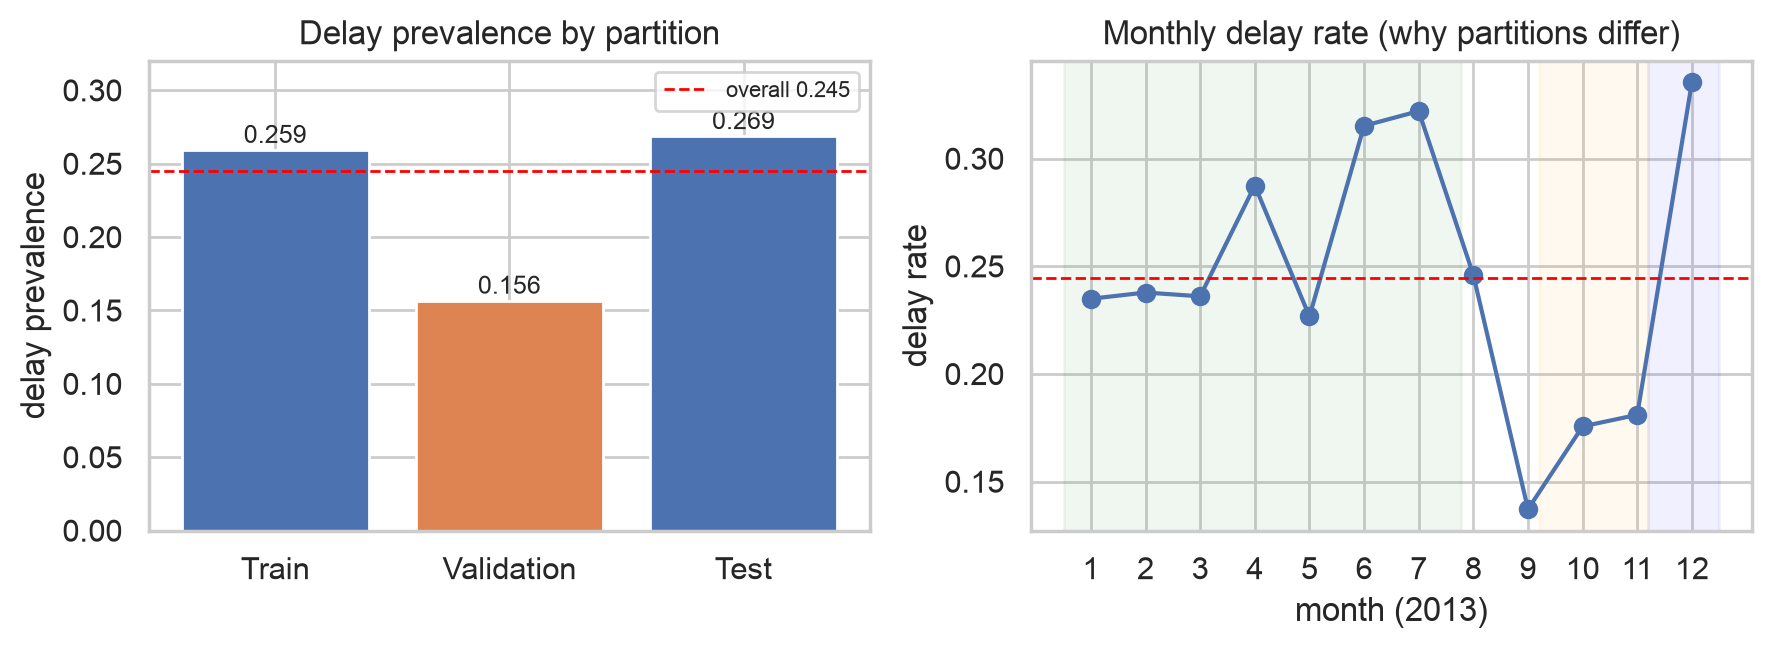
\includegraphics[width=\columnwidth]{prevalence-shift}
  \caption{Delay prevalence by partition (left) and the 2013 monthly delay-rate
  trend (right). The chronological split places the low-delay autumn months in
  validation, so partition prevalences differ by design.}
  \label{fig:prevalence}
\end{figure}

Exploratory analysis, conducted on the training partition only, surfaces the
structure the features are designed to exploit
(Figs.~\ref{fig:target}--\ref{fig:distance}):
\begin{itemize}
  \item \textbf{Time of day.} Delay risk rises monotonically from roughly
  $10.5\%$ for early-morning departures to about $40\%$ late in the evening, as
  delays accumulate and cascade through the day.
  \item \textbf{Seasonality.} Summer is worst (July $\approx 32\%$), September
  best ($\approx 16\%$), reflecting weather and peak-travel load.
  \item \textbf{Day of week.} Weekdays ($27.8\%$) exceed weekends ($20.4\%$).
  \item \textbf{Carrier.} Delay propensity varies widely by operator, from
  $\approx 14\%$ to $\approx 41\%$.
  \item \textbf{Origin.} EWR ($27.9\%$) $>$ JFK ($25.5\%$) $>$ LGA ($24.0\%$),
  and delay risk also varies sharply at the finer route level
  (Fig.~\ref{fig:originroute}).
  \item \textbf{Distance.} Delay rate is largely flat across distance bands and
  dips only for the longest hauls (Fig.~\ref{fig:distance}), confirming that raw
  distance is a weak standalone signal and motivating the route and historical
  features instead.
\end{itemize}

\begin{figure}[t]
  \centering
  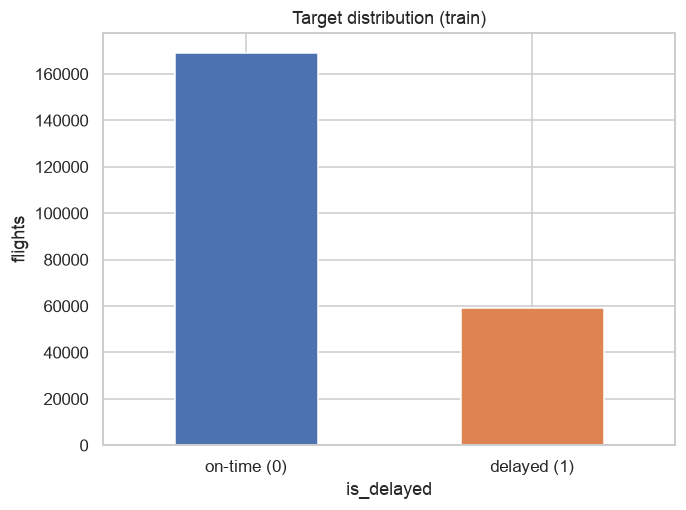
\includegraphics[width=0.78\columnwidth]{target-distribution}
  \caption{Target class balance: delayed versus on-time arrivals. The minority
  (delayed) class motivates PR-AUC and class weighting.}
  \label{fig:target}
\end{figure}

\begin{figure}[t]
  \centering
  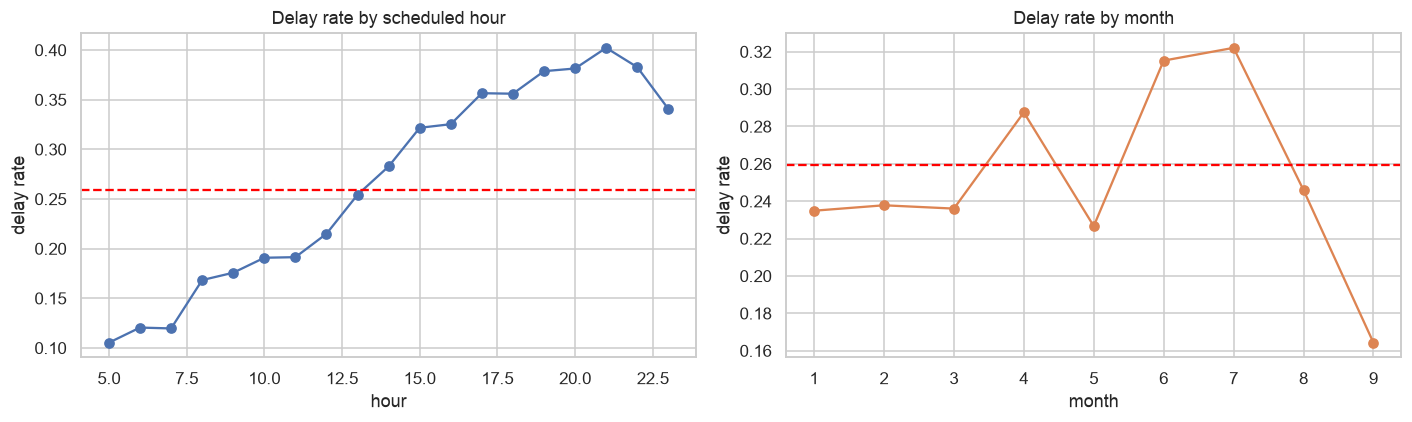
\includegraphics[width=\columnwidth]{delay-hour-month}
  \caption{Delay rate by scheduled hour and month, exposing the strong
  time-of-day and seasonal structure exploited by the temporal features.}
  \label{fig:hourmonth}
\end{figure}

\begin{figure}[t]
  \centering
  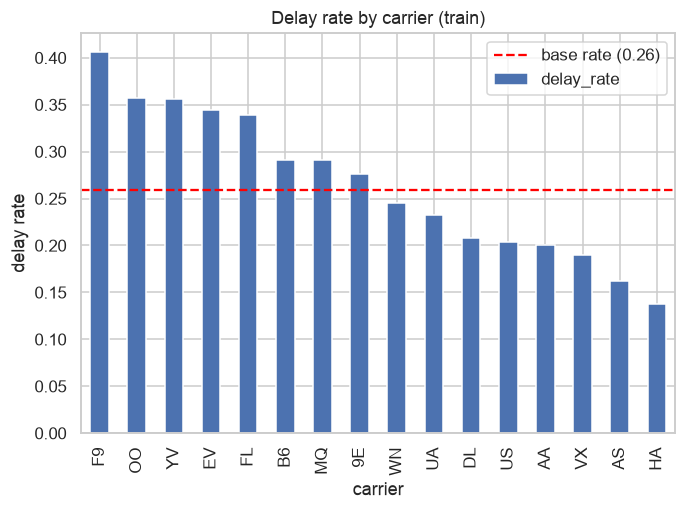
\includegraphics[width=\columnwidth]{delay-carrier}
  \caption{Delay rate by carrier. Operator-level variation motivates the
  carrier historical-delay features.}
  \label{fig:carrier}
\end{figure}

\begin{figure}[t]
  \centering
  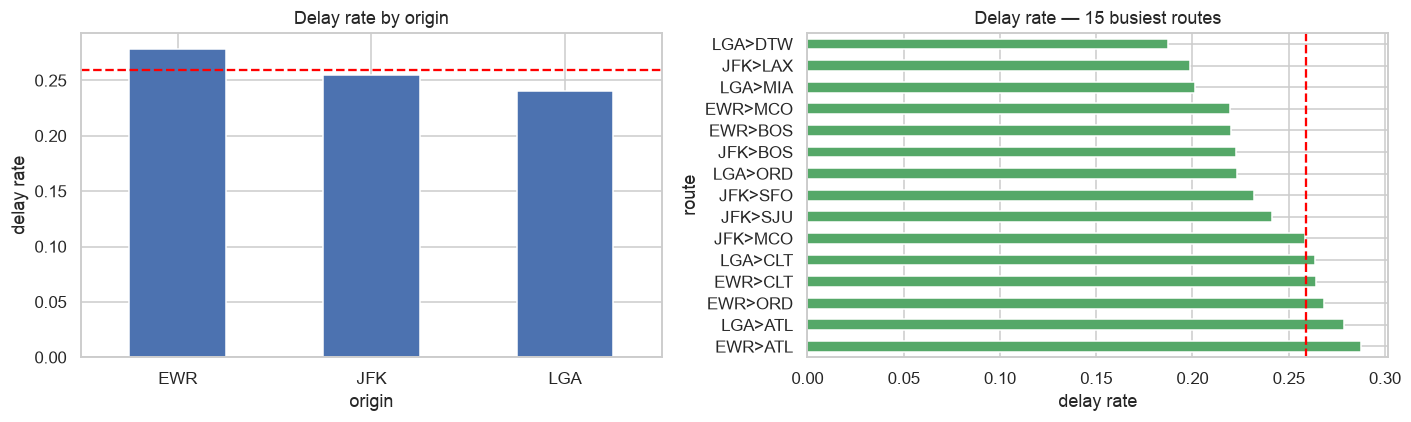
\includegraphics[width=\columnwidth]{delay-origin-route}
  \caption{Delay rate by origin airport (left) and across the fifteen busiest
  origin$\rightarrow$destination routes (right), each against the overall base
  rate (dashed). Route-level spread of roughly $19\%$ to $29\%$ motivates the
  route and route-historical features.}
  \label{fig:originroute}
\end{figure}

\begin{figure}[t]
  \centering
  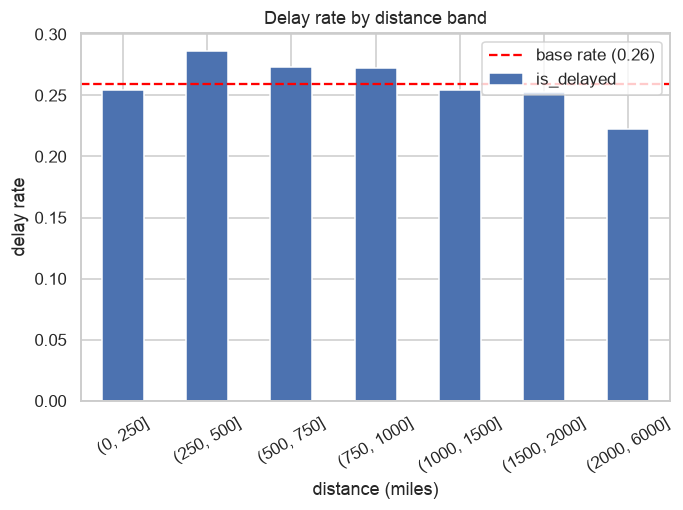
\includegraphics[width=0.82\columnwidth]{delay-distance}
  \caption{Delay rate by binned flight distance. The near-flat profile shows
  distance alone carries little signal, so it enters only as context for the
  route encoding.}
  \label{fig:distance}
\end{figure}

\section{Feature Engineering}
\label{sec:features}
All features derive strictly from the schedule and from historical outcomes on
prior calendar dates, yielding $33$ model features in total. Four engines
contribute, each documented and unit-tested.

\subsection{Temporal features}
Calendar signals (\code{day\_of\_week}, \code{is\_weekend}, \code{season}) are
augmented with a \emph{cyclic} encoding of hour, month and weekday. A raw integer
hour misleads a model because it places $23{:}00$ twenty-three units from
$00{:}00$, although they are one hour apart. Mapping each periodic value $x$ with
period $P$ onto a circle,
\begin{equation}
x \mapsto \left(\sin\tfrac{2\pi x}{P},\ \cos\tfrac{2\pi x}{P}\right),
\end{equation}
restores the true adjacency (Fig.~\ref{fig:cyclic}); linear models in particular
benefit.

\begin{figure}[t]
  \centering
  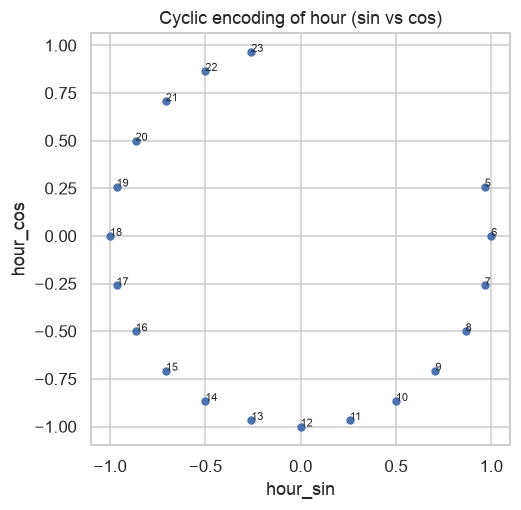
\includegraphics[width=0.82\columnwidth]{cyclic-hour}
  \caption{Cyclic hour encoding: hour $23$ sits adjacent to hour $0$ on the
  circle, unlike the raw integer representation.}
  \label{fig:cyclic}
\end{figure}

\subsection{Route features}
Static route descriptors encode the corridor and its length: the
origin$\rightarrow$destination identifier, a binned \code{distance\_band}, a
long-haul flag ($\geq 1500$ miles) and $\log(1+\text{distance})$ to compress the
heavy tail (the raw distance signal being weak, Fig.~\ref{fig:distance}). These
are fixed regardless of outcome and so introduce no leakage.

\subsection{Historical delay features}
For each carrier, origin, destination and route we compute a historical delay
rate and flight count from \emph{previous calendar dates only}, using a shifted
cumulative aggregation so that same-day and future observations are never
included. These prior-date rates correlate with the target and summarise
congestion and operational reliability that the static features cannot.
Among them, the carrier and route prior-date rates correlate most strongly with
the target (Fig.~\ref{fig:histcorr}), consistent with the operator- and
corridor-level structure seen in the exploratory analysis.
We document openly that this guarantees prior-date ordering but not the
\emph{exact} availability of each outcome at the precise prediction instant;
availability-time leakage therefore remains a stated caveat.

\begin{figure}[t]
  \centering
  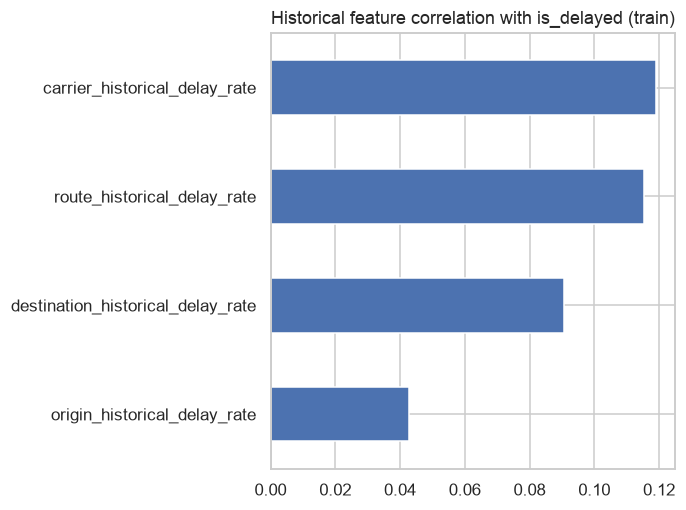
\includegraphics[width=0.9\columnwidth]{hist-correlation}
  \caption{Pearson correlation of each prior-date historical delay rate with the
  target on the training partition. Carrier- and route-level histories are the
  most informative.}
  \label{fig:histcorr}
\end{figure}

\subsection{Airport congestion features}
To represent \emph{airport congestion} directly---rather than only through the
historical volume proxies above---we add two schedule-derived counts:
\code{origin\_hourly\_departures}, the number of flights scheduled to depart the
same origin in the same (date, hour), and \code{dest\_hourly\_arrivals}, the
analogous scheduled arrival load at the destination. Both are read from the
timetable, so they are known before any flight departs and introduce no leakage.
On this dataset their marginal value is small: they rank low in model importance
(below the top~30 encoded features) and are weakly, negatively correlated with
delay, because the scheduled hour already captures most of the time-of-day
congestion structure. We include them for completeness and because a larger,
multi-airport dataset would likely make an explicit congestion signal more
informative.

\subsection{The pre-departure allowlist}
A single feature contract admits only approved predictors
(schedule, route, historical, congestion) into the design matrix and blocks the
target, every post-departure column, and identifiers. The contract is enforced in
code and in tests, so leakage cannot enter by accident.

\section{Methodology}
\label{sec:method}
\subsection{Chronological split and calibration windows}
The data are partitioned by \emph{distinct calendar date} into train/validation/
test at $70/15/15$, so all flights on a date stay together and training dates
strictly precede validation dates, which precede test dates. For calibration,
the training period is split again in time: the earliest $80\%$ of training dates
fit the base estimator and preprocessing (the \emph{base-train} window), and the
remaining $20\%$ fit the calibrator (the \emph{calibration} window). No
calibration-window label ever fits a base estimator. The resulting windows are
summarised in Table~\ref{tab:windows}.

\begin{table}[t]
  \caption{Chronological windows (2013).}
  \label{tab:windows}
  \centering
  \begin{tabular}{lrll}
    \toprule
    Window & $n$ & First & Last \\
    \midrule
    Base train        & $181{,}405$ & Jan 1  & Jul 23 \\
    Calibration        & $46{,}894$  & Jul 24 & Sep 12 \\
    Validation         & $50{,}466$  & Sep 13 & Nov 6  \\
    Test (held out)    & $48{,}581$  & Nov 7  & Dec 31 \\
    \bottomrule
  \end{tabular}
\end{table}

\subsection{Models}
Two classifiers share the identical training rows and feature contract:
\begin{itemize}
  \item \textbf{Logistic Regression} with \code{class\_weight="balanced"} to
  counter the class imbalance.
  \item \textbf{Tuned XGBoost} with parameters selected previously by
  training-only chronological cross-validation: $250$ trees, max depth $6$,
  learning rate $0.03$, minimum child weight $10$, subsample $0.90$, column
  subsample $0.75$, $L_2$ regularisation $10$, and
  \code{scale\_pos\_weight}$\,\approx 2.86$ for imbalance.
\end{itemize}
This XGBoost configuration was selected by \code{RandomizedSearchCV} over eight
sampled candidates on the \emph{training data only}, scored with three expanding
chronological folds grouped by whole flight dates and separated by a one-date
embargo so that no fold shares a date across the train/validation boundary. The
search ranged over tree count, depth, learning rate, minimum child weight, row
and column subsampling, $L_2$ regularisation and positive-class weighting; the
held-out test set was never consulted.

\subsection{Calibration}
Each model's calibration-window scores are mapped by three candidates---raw
(identity), sigmoid (Platt)~\cite{platt}, and isotonic~\cite{zadrozny}---and the
variant minimising validation Brier score (log loss as tie-break) is selected.
Calibrators are fit strictly on the calibration window; validation and test
labels never fit them.

\subsection{Threshold selection and the frozen protocol}
A single operating threshold per model is chosen on validation (maximising $F_1$;
precision-floor variants are reported only as illustrative sensitivity, as no
operational cost was approved). The selected calibration map and threshold, the
fitted estimators, the dataset hash and the dependency versions are then
\emph{frozen} to disk. Only after this does the final stage load the frozen
objects and evaluate the held-out test set \emph{exactly once}; it cannot refit
or reselect. This discipline prevents the test set from leaking into any
modelling decision.

\section{Results}
\label{sec:results}
\subsection{Validation}
Table~\ref{tab:val} reports validation performance at the frozen thresholds with
the selected (isotonic) calibration for both models. Ranking is similar; both
models have low precision ($\approx 22\%$) at their operating points, reflecting
the difficulty of the task. ROC and PR curves appear in
Figs.~\ref{fig:roc}--\ref{fig:pr}, and the confusion matrices at the frozen
thresholds in Fig.~\ref{fig:confusion}. On validation alone the balanced LR in
fact edges XGBoost, and its PR-AUC advantage is marginally significant under the
date-block bootstrap (Section~\ref{sec:results}\,C); the ROC-AUC and $F_1$ gaps
are not. Because this ordering reverses on the held-out test, we defer the model
choice to that one-time test (Section~\ref{sec:results}\,C), where XGBoost is the
stronger candidate on every metric. Both operating points favour recall over precision---catching
roughly $60\%$ of true delays at the cost of a large false-alarm count
(Fig.~\ref{fig:confusion})---which is the intended behaviour under class
weighting and is exactly what the cost analysis of Section~\ref{sec:resched}
later prices.

\begin{figure}[t]
  \centering
  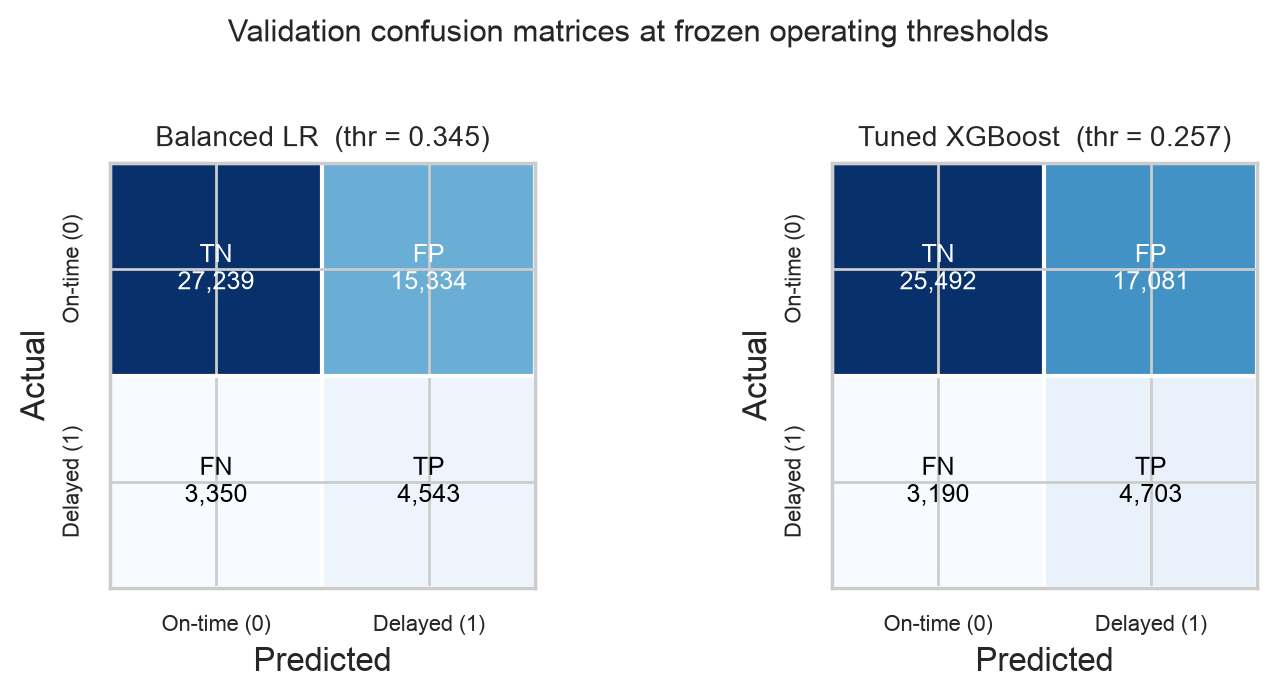
\includegraphics[width=\columnwidth]{confusion}
  \caption{Validation confusion matrices at the frozen operating thresholds.
  Both models recover a majority of true delays (high recall) while incurring
  many false positives, consistent with their low operating precision.}
  \label{fig:confusion}
\end{figure}

\begin{table}[t]
  \caption{Validation metrics (isotonic calibration; frozen thresholds).}
  \label{tab:val}
  \centering
  \setlength{\tabcolsep}{4pt}
  \resizebox{\columnwidth}{!}{%
  \begin{tabular}{lrrrrrr}
    \toprule
    Model & Thr. & PR-AUC & ROC-AUC & Prec. & Rec. & Brier \\
    \midrule
    Balanced LR    & $0.345$ & $0.230$ & $0.638$ & $0.229$ & $0.576$ & $0.152$ \\
    Tuned XGBoost  & $0.257$ & $0.212$ & $0.626$ & $0.216$ & $0.596$ & $0.137$ \\
    \bottomrule
  \end{tabular}}
\end{table}

\begin{figure}[t]
  \centering
  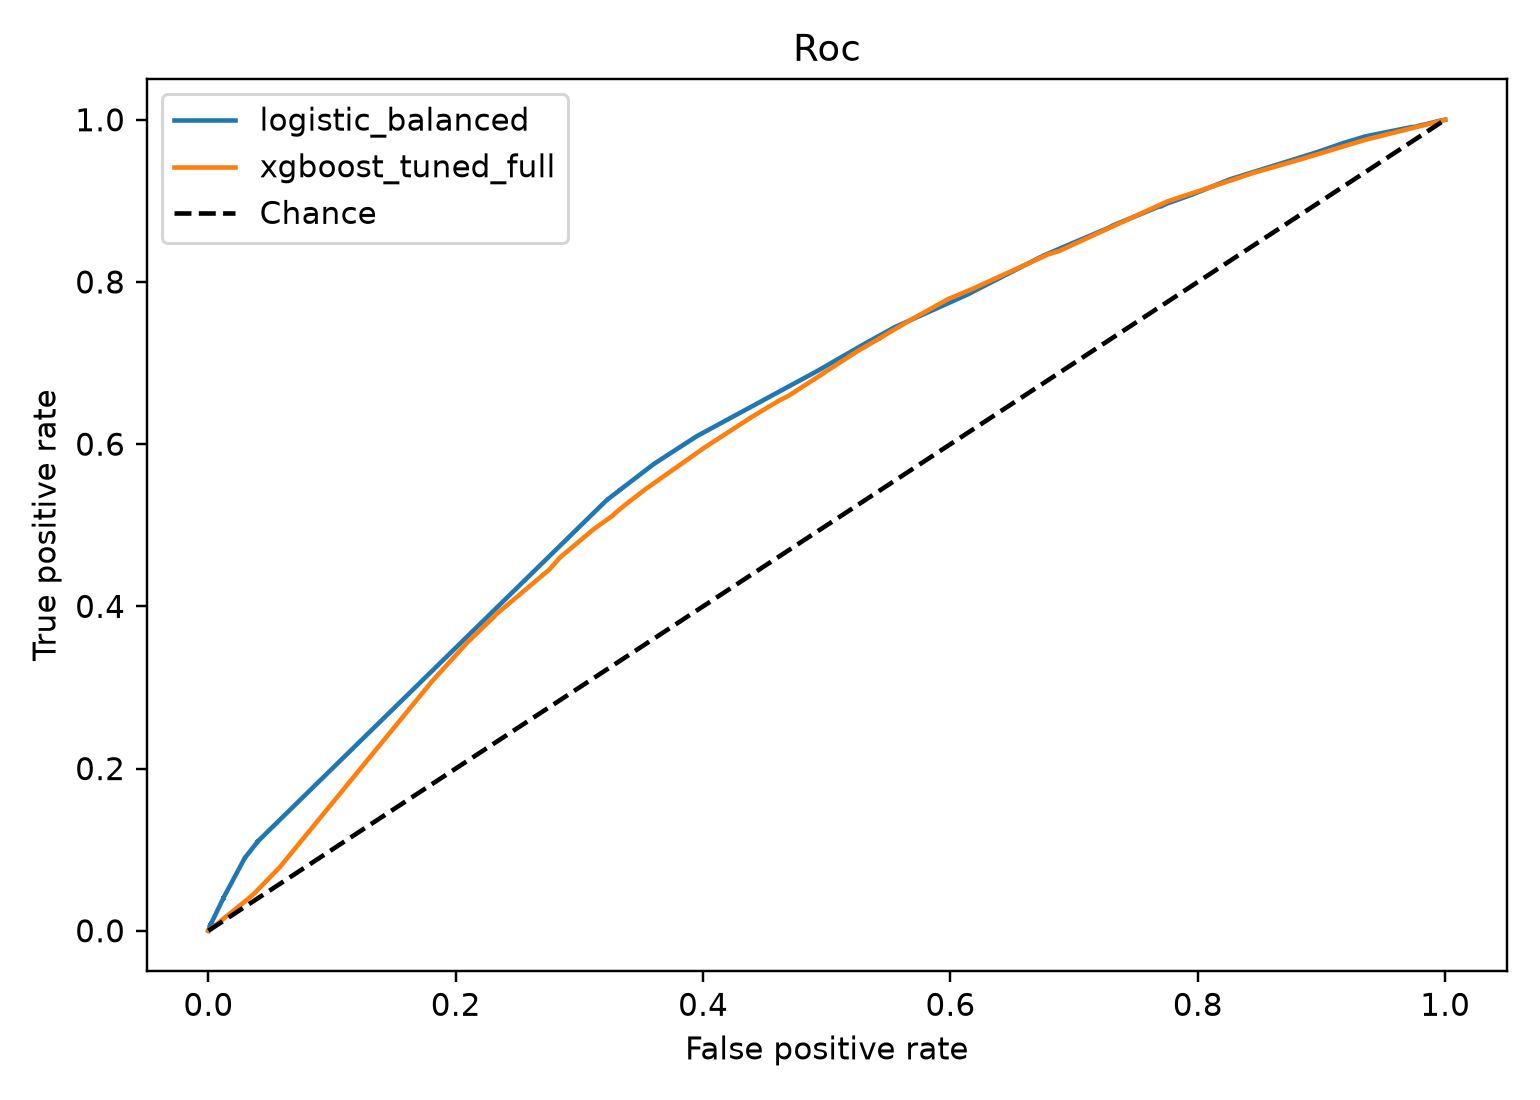
\includegraphics[width=\columnwidth]{val-roc}
  \caption{Validation ROC curves. Discrimination is modest in absolute terms
  (ROC-AUC $\approx 0.63$).}
  \label{fig:roc}
\end{figure}

\begin{figure}[t]
  \centering
  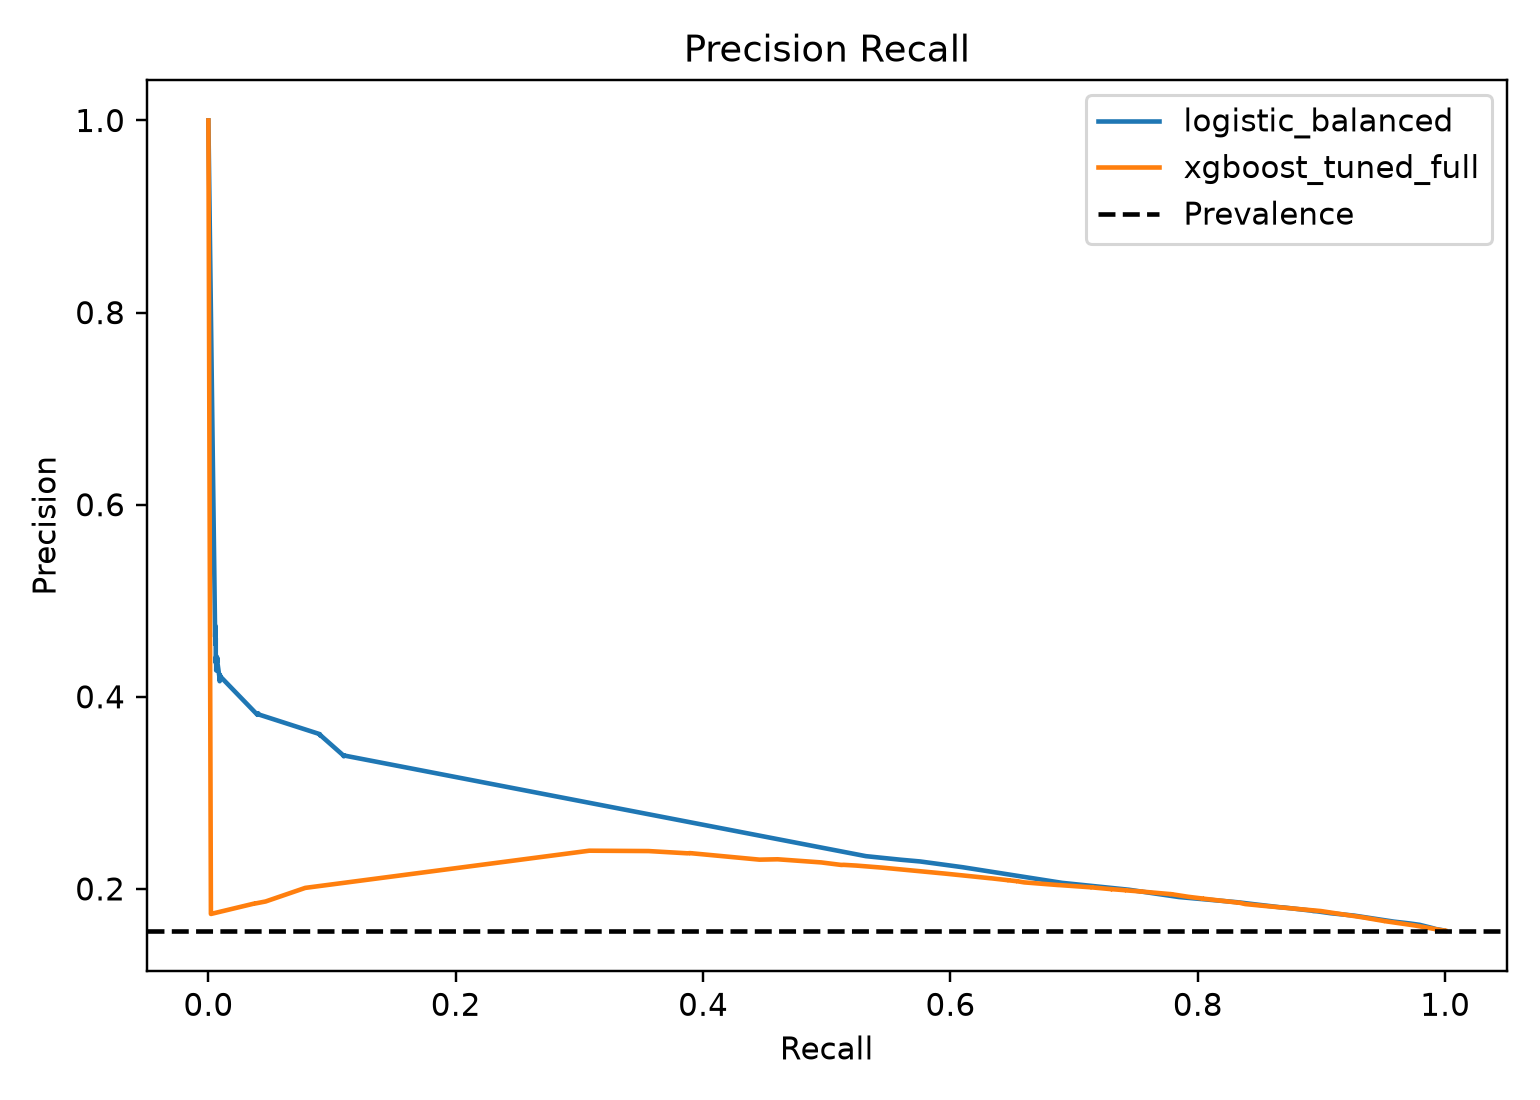
\includegraphics[width=\columnwidth]{val-pr}
  \caption{Validation precision--recall curves against the prevalence
  no-skill reference.}
  \label{fig:pr}
\end{figure}

\subsection{Calibration quality}
Isotonic regression minimises validation Brier and log loss for both models and
is selected. A proper-score audit, however, tempers any success claim: a constant
predictor set to the late-training prevalence attains a Brier of $0.138$, which
the balanced-LR isotonic probabilities ($0.152$) \emph{fail} to beat and the
XGBoost isotonic probabilities ($0.137$) beat only narrowly. Improvement over
severely miscalibrated raw scores is therefore not sufficient evidence of useful
probability forecasts. Table~\ref{tab:calib} reports the proper scores and the
mean predicted probability for both models before and after calibration:
calibration slashes Brier and log loss, yet the calibrated mean prediction
($0.23$--$0.31$) still sits above the observed validation prevalence ($0.156$),
i.e.\ both models over-predict on this lower-prevalence window---another reason
the calibrated probabilities are only modestly useful. The XGBoost reliability
diagram (Fig.~\ref{fig:reliability}) is reasonable but not strong.

\begin{table}[t]
  \caption{Validation calibration quality (observed prevalence $0.156$;
  prevalence-baseline Brier $0.138$). Lower Brier/log loss is better; a
  well-calibrated mean prediction would match the observed prevalence.}
  \label{tab:calib}
  \centering
  \setlength{\tabcolsep}{4pt}
  \begin{tabular}{llrrr}
    \toprule
    Model & Variant & Brier & Log loss & Mean pred. \\
    \midrule
    Balanced LR   & raw       & $0.520$ & $1.389$ & $0.780$ \\
    Balanced LR   & isotonic  & $0.152$ & $0.518$ & $0.308$ \\
    Tuned XGBoost & raw       & $0.303$ & $0.850$ & $0.537$ \\
    Tuned XGBoost & isotonic  & $\mathbf{0.137}$ & $\mathbf{0.442}$ & $0.231$ \\
    \bottomrule
  \end{tabular}
\end{table}

\begin{figure}[t]
  \centering
  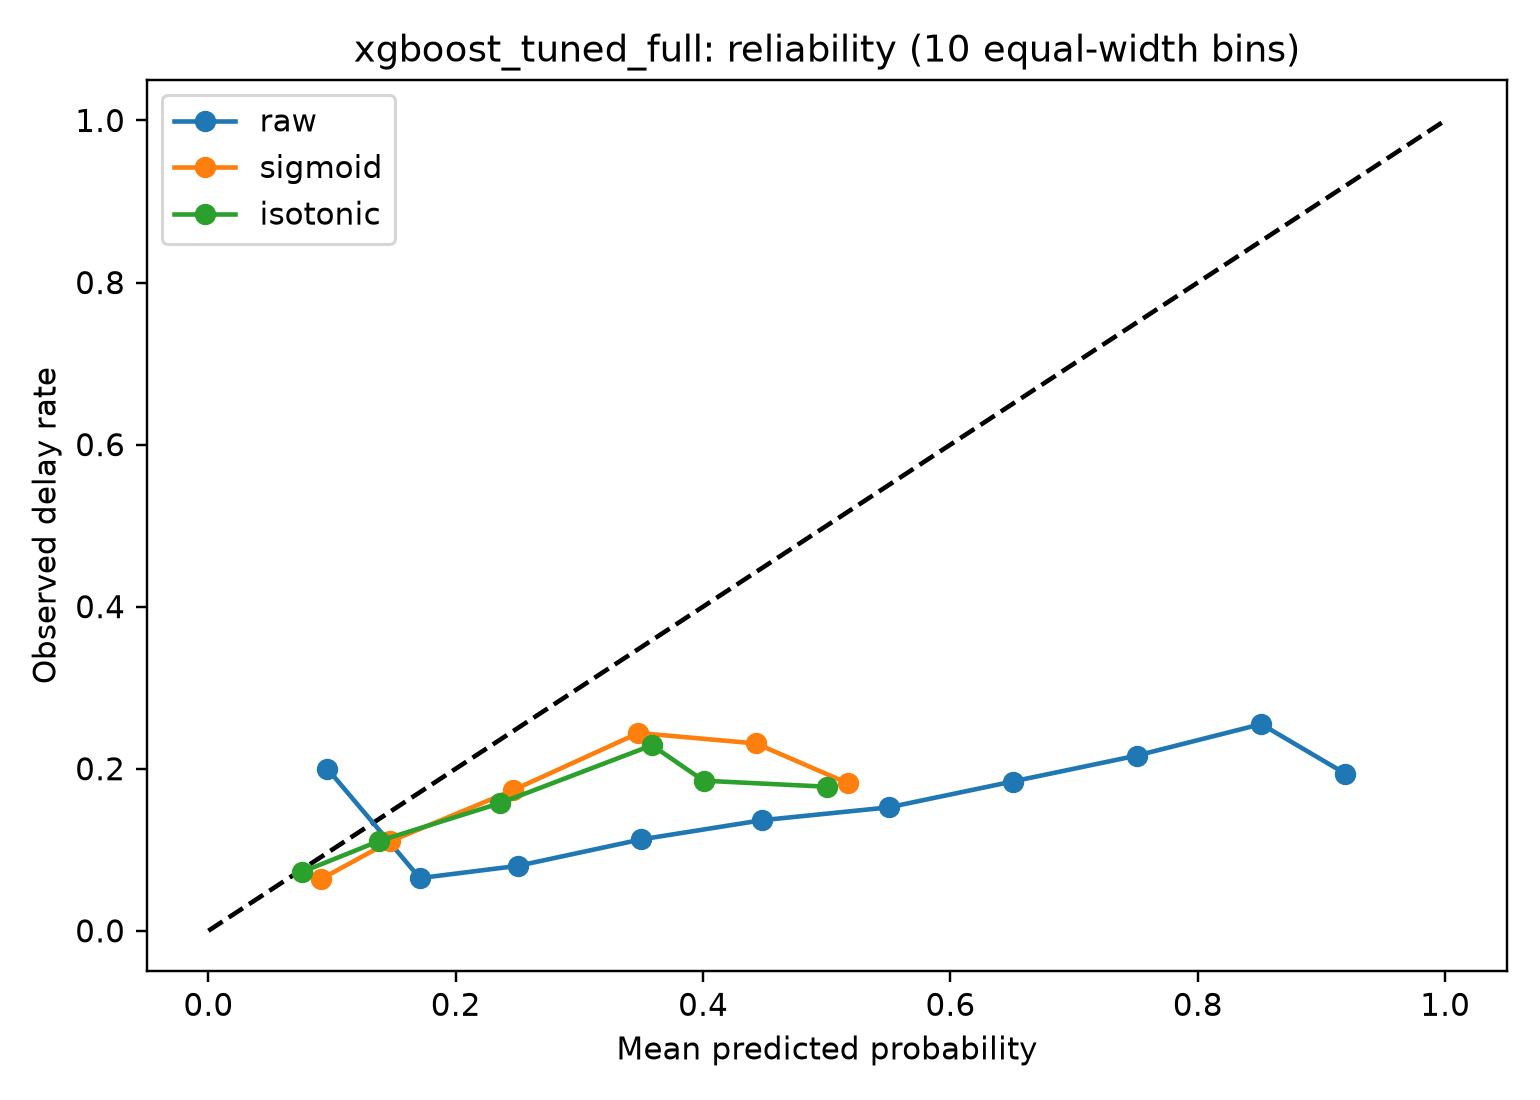
\includegraphics[width=0.9\columnwidth]{xgb-reliability}
  \caption{Validation reliability diagram for the calibrated XGBoost model
  (ten equal-width bins).}
  \label{fig:reliability}
\end{figure}

\subsection{Held-out test}
The frozen one-time test (Table~\ref{tab:test}) favours XGBoost on PR-AUC,
ROC-AUC, precision, recall and $F_1$. Because prevalence differs between
validation ($0.156$) and test ($0.269$), the two sets' PR-based metrics are not
directly comparable as measures of improvement. The comparison is also
window-dependent: a paired date-block bootstrap on \emph{validation} (300
resamples) gives differences (XGBoost minus LR) whose $95\%$ intervals favour LR
on PR-AUC ($[-0.033, -0.001]$, excluding zero) but include zero for ROC-AUC
($[-0.029, 0.005]$) and $F_1$ ($[-0.022, 0.005]$). On the held-out test the
ordering reverses and XGBoost leads on every metric. The between-model difference
is therefore window-dependent and, on balance, not robustly established in
either model's favour; we select XGBoost on the held-out test and its cost
behaviour (Section~\ref{sec:resched}), not on a significant ranking gap.

\begin{table}[t]
  \caption{Held-out test metrics (frozen one-time evaluation).}
  \label{tab:test}
  \centering
  \setlength{\tabcolsep}{4pt}
  \resizebox{\columnwidth}{!}{%
  \begin{tabular}{lrrrrr}
    \toprule
    Model & PR-AUC & ROC-AUC & Prec. & Rec. & $F_1$ \\
    \midrule
    Balanced LR    & $0.296$ & $0.545$ & $0.300$ & $0.465$ & $0.364$ \\
    Tuned XGBoost  & $\mathbf{0.338}$ & $\mathbf{0.599}$ & $\mathbf{0.332}$ & $\mathbf{0.542}$ & $\mathbf{0.412}$ \\
    \bottomrule
  \end{tabular}}
\end{table}

\subsection{Feature importance}
The tuned XGBoost model's gain-importance ranking (Fig.~\ref{fig:importance})
is dominated by time-of-day signals: scheduled \code{hour}, its cyclic
\code{hour\_sin} encoding and \code{sched\_dep\_time} account for the largest
share, followed by the \code{season} flag and a high-delay carrier indicator.
This agrees with the exploratory finding that delay risk is primarily driven by
when a flight departs (Figs.~\ref{fig:hourmonth}), and confirms that the
engineered temporal features carry real model weight rather than mere decoration.
The explicit congestion counts, by contrast, rank well outside the top ten,
confirming that the scheduled hour already absorbs most time-of-day congestion.
Importance here is model-relative and does not imply causation; correlated
calendar features can share or dilute one another's attributed gain.

\begin{figure}[t]
  \centering
  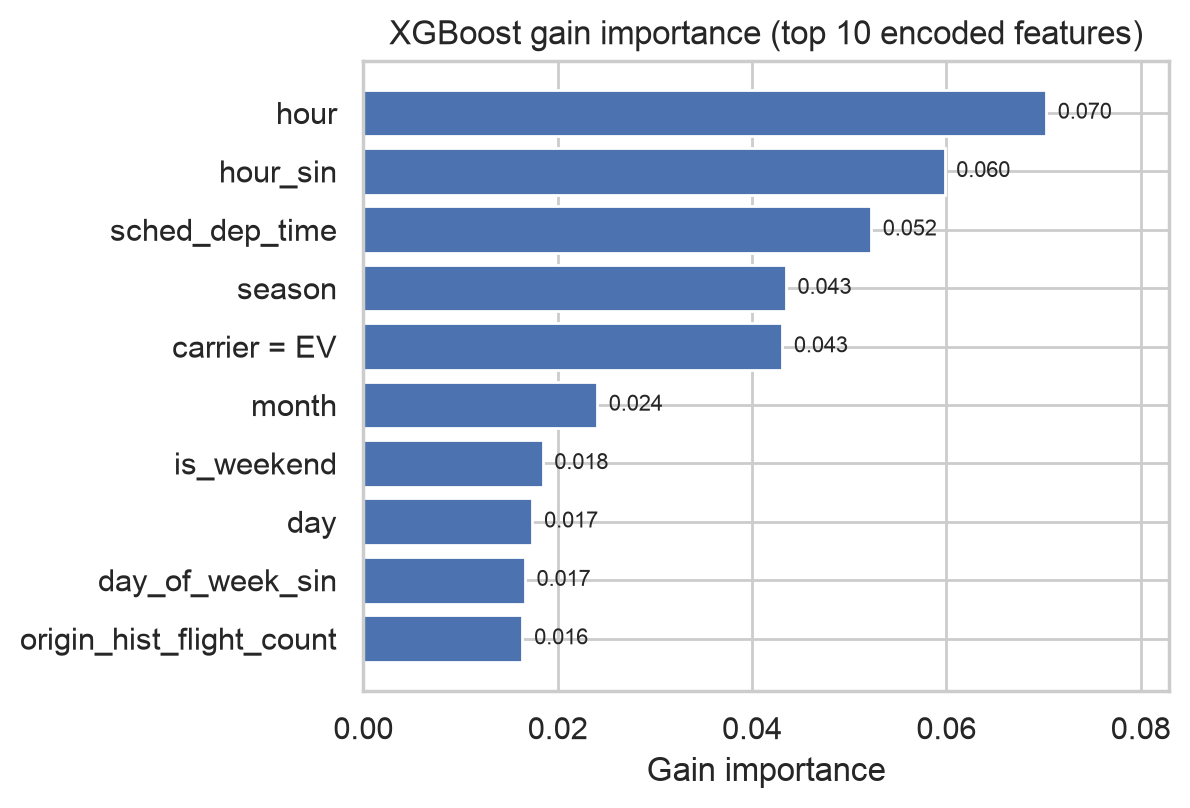
\includegraphics[width=0.95\columnwidth]{xgb-importance}
  \caption{XGBoost gain importance for the ten most influential encoded
  features. Time-of-day terms dominate, matching the exploratory structure.}
  \label{fig:importance}
\end{figure}

\section{Offline Rescheduling What-If Analysis}
\label{sec:resched}
\subsection{Cost model}
We ask, retrospectively, what the net operational cost would have been had a
proactive rescheduling action been taken on flights whose calibrated delay
probability exceeds a threshold. Per flight we assume homogeneous costs: $C_d$
for an unmitigated delay, $C_a$ for taking the action (paid whenever we act), and
a recovery fraction $r\in[0,1]$ of the delay cost avoided when we act on a flight
that truly delays. The realised cost by decision $a$ and outcome $y$ is
\begin{center}
\begin{tabular}{lcc}
\toprule
 & $y=0$ (on time) & $y=1$ (delayed) \\
\midrule
$a=0$ (no action) & $0$ & $C_d$ \\
$a=1$ (action)    & $C_a$ & $C_a + (1-r)C_d$ \\
\bottomrule
\end{tabular}
\end{center}
These assumptions---homogeneous per-flight costs, independent flights, a single
binary action, and no network feedback---are strong and are declared as
limitations; no operational cost has been approved, so all quantities are
expressed relative to $C_d$.

\subsection{Closed-form net benefit and the optimal threshold}
For a policy that acts on $\mathrm{tp}$ true delays and $\mathrm{fp}$ on-time
flights, the saving relative to the no-action status quo is
\begin{equation}
\text{net} = \mathrm{tp}\,(r\,C_d - C_a) - \mathrm{fp}\,C_a,
\label{eq:net}
\end{equation}
a cost-sensitive generalisation of decision-curve net benefit~\cite{vickers}.
Acting on a flight has non-negative expected value exactly when its calibrated
probability $p$ satisfies $p\,r\,C_d \geq C_a$, giving the \emph{cost-optimal
action threshold}
\begin{equation}
\tau^\star = \frac{C_a}{r\,C_d} = \frac{C_a/C_d}{r}.
\label{eq:tau}
\end{equation}
The decision boundary is thus read directly from the cost assumptions---which is
precisely why calibration matters operationally, as only a well-calibrated $p$
makes $\tau^\star$ the right place to cut.

\subsection{Sensitivity and findings}
Because real costs are unknown, we sweep the cost ratio $C_a/C_d$ at
$r=0.8$ on the validation partition (preserving the held-out test), evaluating
each model at its optimal $\tau^\star$ (Table~\ref{tab:sweep},
Fig.~\ref{fig:netbenefit}).

\begin{table}[t]
  \caption{Rescheduling sensitivity: net saving per flight (units of $C_d$) at
  the cost-optimal threshold, $r=0.8$. ``$+$'' beats no action.}
  \label{tab:sweep}
  \centering
  \begin{tabular}{rrrr}
    \toprule
    $C_a/C_d$ & $\tau^\star$ & Balanced LR & Tuned XGBoost \\
    \midrule
    $0.05$ & $0.063$ & $+0.075$ & $+0.075$ \\
    $0.10$ & $0.125$ & $+0.025$ & $+0.034$ \\
    $0.15$ & $0.188$ & $-0.016$ & $+0.005$ \\
    $0.20$ & $0.250$ & $-0.046$ & $-0.012$ \\
    $0.25$ & $0.313$ & $-0.049$ & $-0.020$ \\
    \bottomrule
  \end{tabular}
\end{table}

\begin{figure}[t]
  \centering
  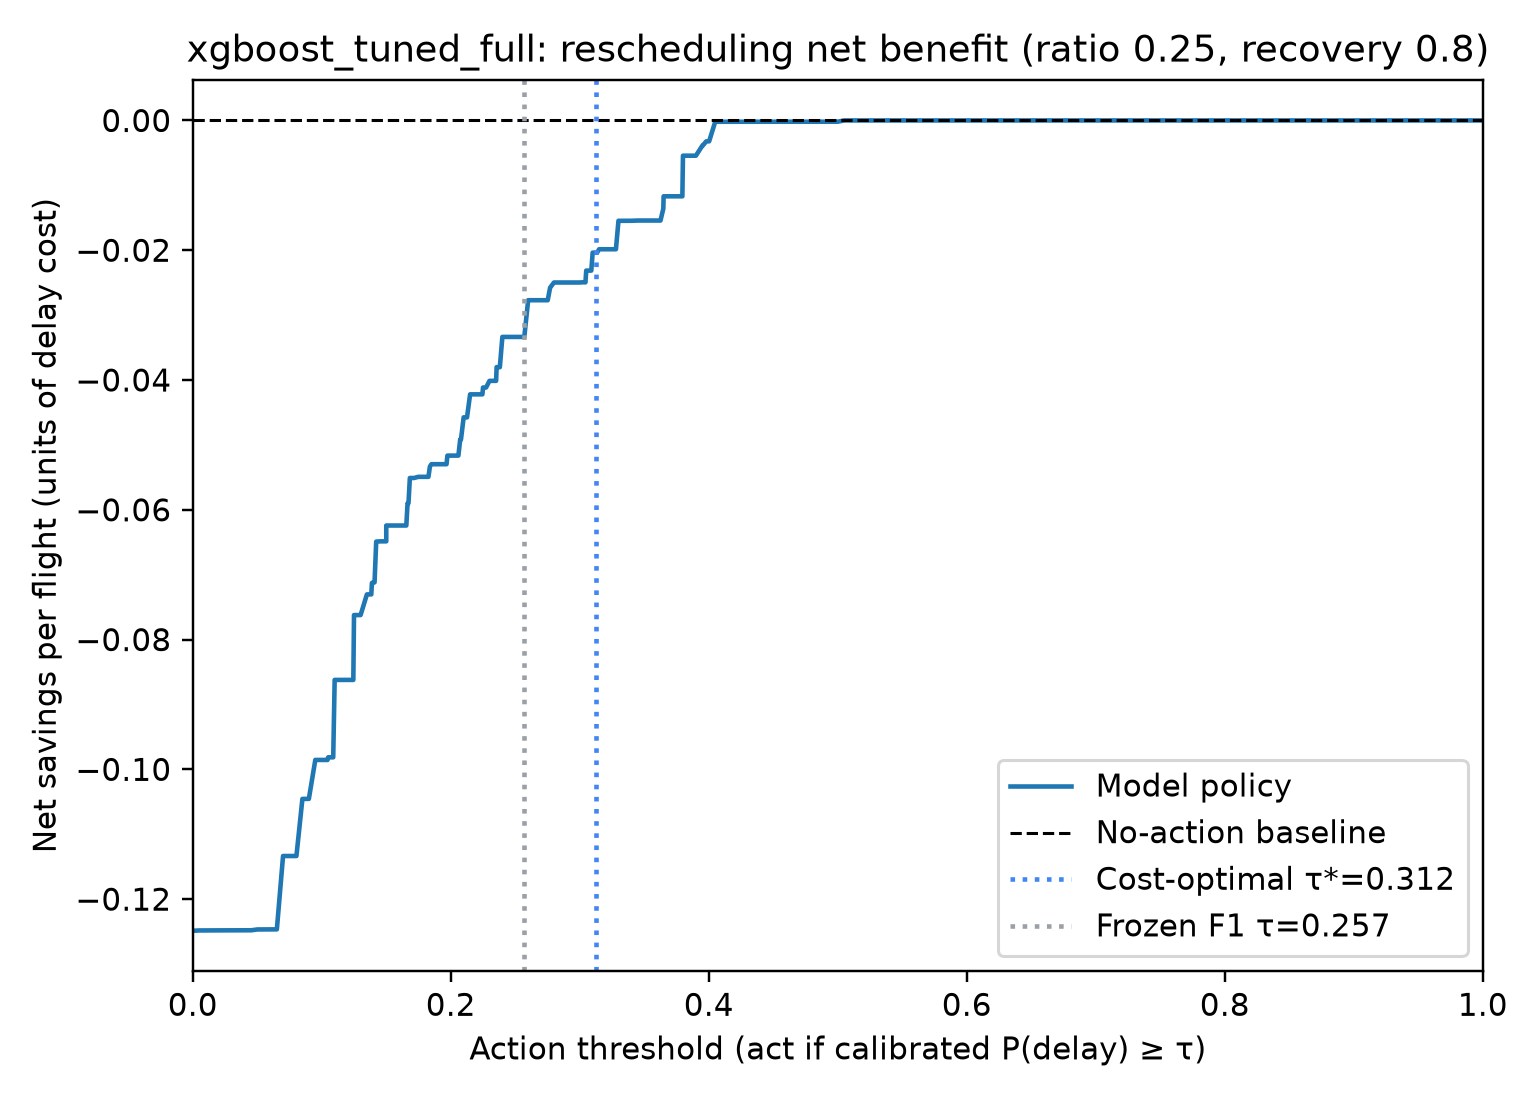
\includegraphics[width=\columnwidth]{xgb-netbenefit}
  \caption{XGBoost net saving per flight versus action threshold. The curve
  crosses the no-action line, and the cost-optimal $\tau^\star$ moves with the
  assumed cost ratio.}
  \label{fig:netbenefit}
\end{figure}

Three findings follow. First, a model-driven rule beats inaction only when the
action is cheap relative to a delay---up to $C_a/C_d\approx 0.10$ for Logistic
Regression and $\approx 0.15$ for XGBoost; beyond that, low precision makes the
false-alarm term in~\eqref{eq:net} dominate and intervention is not justified.
Second, \textbf{XGBoost has the more favourable sensitivity profile across the
meaningful cost range}---a wider contiguous positive-saving region (profitable up
to $C_a/C_d\approx 0.15$ versus $\approx 0.10$ for Logistic Regression) and higher
oracle efficiency at matched cost ratios---a decision-relevant advantage the
ranking metrics alone did not make vivid. The single exception is a degenerate
high-cost point ($C_a/C_d=0.30$), where Logistic Regression records a negligible
positive saving only because its calibrated scores rarely clear the high
threshold and it therefore acts on almost no flights; this is not a meaningful
reversal. Third, even the best attainable efficiency is modest (about $64\%$ of the
perfect-foresight oracle at the cheapest ratio), bounding what any policy built on
the current probabilities can deliver.

\section{Discussion and Limitations}
\label{sec:discussion}
The results are deliberately unembellished. Discrimination is modest
(ROC-AUC $\approx 0.60$), the calibrated probabilities barely improve on a
prevalence baseline in proper-score terms, and the between-model difference is
not statistically established. This ceiling is, however, largely expected rather
than a modelling failure: by construction the predictor sees only schedule,
route and prior-date history, and is denied the single strongest driver of
day-of-operation delay---weather---together with real-time congestion and
upstream-aircraft state, none of which is available at the pre-departure
decision point we committed to. The gain-importance ranking
(Fig.~\ref{fig:importance}) reflects exactly this: the model extracts what
temporal and historical structure it can, but that structure bounds how far any
pre-departure classifier on this feature set can go. We therefore read
ROC-AUC $\approx 0.60$ as an honest estimate of the information actually present
before departure, not as an artefact of weak modelling. The rescheduling analysis shows a genuine but
narrow operating regime. Key limitations: (i) historical features guarantee
prior-date ordering but not exact availability-time safety; (ii) the data cover a
single year and only three New York origin airports, limiting generalisation;
(iii) the calibration study is conditional on hyperparameters chosen over the
full original training period and is not fully nested; (iv) the rescheduling
cost model assumes homogeneous, independent per-flight costs with no network
feedback; (v) delay prevalence shifts substantially across the chronological
partitions (Fig.~\ref{fig:prevalence}), so prevalence-dependent metrics are not
directly comparable across windows; and (vi) the explicit scheduled-congestion
features add little here (single hub region, one year), so their value remains to
be demonstrated on a larger multi-airport dataset. None of the
results supports a production-readiness claim.

\section{Conclusion and Future Work}
\label{sec:conclusion}
We delivered a leakage-safe, calibrated and honestly evaluated baseline for
pre-departure flight-delay prediction, together with an offline rescheduling
what-if analysis grounded in explicit cost assumptions. XGBoost is the stronger
descriptive candidate and the better basis for a cost-sensitive rescheduling
rule, which nonetheless pays off only under cheap-intervention assumptions.

The deep-learning phase will extend this baseline with learned entity embeddings
for airline, origin and destination, and an optional temporal sequence model over
correctly ordered flight history, benchmarked against the calibrated classical
models reported here on the same chronological protocol and metrics. The larger
BTS on-time dataset offers a route to broader geographic coverage and a sterner
test of generalisation.

\section*{Reproducibility}
The pipeline, models, evaluation and rescheduling analysis are implemented as a
tested Python package (\code{random\_seed}$=42$), with $223$ passing automated
tests and a continuous-integration workflow. The frozen evaluation records the
dataset and artifact SHA-256 hashes and the exact dependency versions, so a
reviewer can confirm that the reported numbers came from the committed data and
code; the final test stage is additionally guarded so it cannot be silently
re-run or re-selected.

\begin{thebibliography}{00}
\bibitem{bts} US Bureau of Transportation Statistics, ``Airline On-Time
Performance Data,'' BTS, TranStats database. [Online]. Available:
\url{https://www.transtats.bts.gov/}
\bibitem{guo} C. Guo, G. Pleiss, Y. Sun, and K. Q. Weinberger, ``On calibration
of modern neural networks,'' in \emph{Proc. 34th Int. Conf. Machine Learning
(ICML)}, 2017, pp. 1321--1330.
\bibitem{xgboost} T. Chen and C. Guestrin, ``XGBoost: A scalable tree boosting
system,'' in \emph{Proc. 22nd ACM SIGKDD Int. Conf. Knowledge Discovery and Data
Mining}, 2016, pp. 785--794.
\bibitem{platt} J. Platt, ``Probabilistic outputs for support vector machines and
comparisons to regularized likelihood methods,'' in \emph{Advances in Large
Margin Classifiers}, 1999, pp. 61--74.
\bibitem{zadrozny} B. Zadrozny and C. Elkan, ``Transforming classifier scores
into accurate multiclass probability estimates,'' in \emph{Proc. 8th ACM SIGKDD
Int. Conf. Knowledge Discovery and Data Mining}, 2002, pp. 694--699.
\bibitem{niculescu} A. Niculescu-Mizil and R. Caruana, ``Predicting good
probabilities with supervised learning,'' in \emph{Proc. 22nd Int. Conf. Machine
Learning (ICML)}, 2005, pp. 625--632.
\bibitem{davis} J. Davis and M. Goadrich, ``The relationship between
precision-recall and ROC curves,'' in \emph{Proc. 23rd Int. Conf. Machine
Learning (ICML)}, 2006, pp. 233--240.
\bibitem{saito} T. Saito and M. Rehmsmeier, ``The precision-recall plot is more
informative than the ROC plot when evaluating binary classifiers on imbalanced
datasets,'' \emph{PLoS ONE}, vol. 10, no. 3, e0118432, 2015.
\bibitem{vickers} A. J. Vickers and E. B. Elkin, ``Decision curve analysis: a
novel method for evaluating prediction models,'' \emph{Medical Decision Making},
vol. 26, no. 6, pp. 565--574, 2006.
\bibitem{sklearn} F. Pedregosa \emph{et al.}, ``Scikit-learn: Machine learning in
Python,'' \emph{J. Machine Learning Research}, vol. 12, pp. 2825--2830, 2011.
\bibitem{rebollo} J. J. Rebollo and H. Balakrishnan, ``Characterization and
prediction of air traffic delays,'' \emph{Transportation Research Part C},
vol. 44, pp. 231--241, 2014.
\bibitem{gui} G. Gui \emph{et al.}, ``Flight delay prediction based on aviation
big data and machine learning,'' \emph{IEEE Trans. Vehicular Technology},
vol. 69, no. 1, pp. 140--150, 2020.
\end{thebibliography}

\end{document}
